\chapter{La gestion de version}

\section{Git : le gestionnaire de code source}

Les logiciels de gestion de versions ou VCS\, \footnote{\emph{Version Control
System.}} sont utilisés principalement par les développeurs. En effet, ils sont
quasi exclusivement utilisés pour gérer des codes sources, car ils sont
capables de suivre l’évolution d’un fichier texte \emph{ligne de code par ligne de
code.} Ces logiciels sont fortement conseillés pour gérer un projet
informatique.

Ils retiennent qui a effectué chaque modification de chaque fichier et
pourquoi. Ils sont par conséquent capables de dire qui a écrit chaque ligne de
chaque fichier et dans quel but ; si deux personnes travaillent simultanément
sur un même fichier, ils sont capables d’assembler (de fusionner) leurs
modifications et d’éviter que le travail d’une de ces personnes ne soit écrasé.

Ces logiciels ont donc par conséquent deux utilités principales :
\begin{itemize}
    \item suivre l’évolution d’un code source, pour retenir les modifications
effectuées sur chaque fichier et être ainsi capable de revenir en arrière en
cas de problème ;
    \item travailler à plusieurs, sans risquer de se marcher sur les pieds.
Si deux personnes modifient un même fichier en même temps, leurs modifications
doivent pouvoir être fusionnées sans perte d’information.
\end{itemize}

Chaque utilisateur possède une copie du code source ainsi que toutes les
versions précédentes de celui-ci, ce qui n'est pas le cas de l'existant. La
figure \ref{workflow} en  page \pageref{workflow} illustre bien le
fonctionnement global de Git.

\begin{figure}
\begin{center}
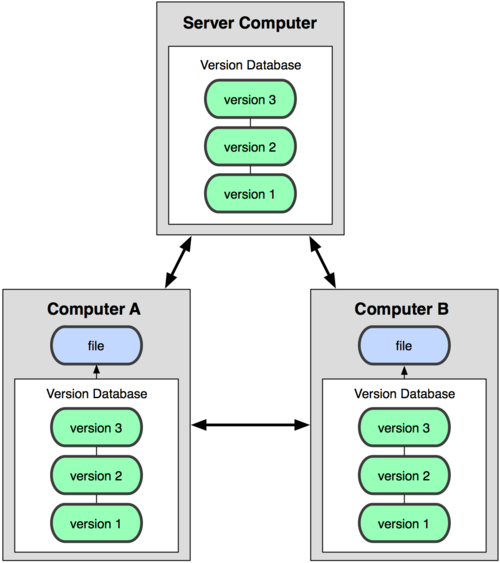
\includegraphics[scale=0.8]{images/workflow.png}
\caption{Le serveur sert de point de rencontre entre les développeurs et possède
lui aussi l’historique des versions.}
\label{workflow}
\end{center}
\end{figure}

\subsection{Les rudiments}

\emph{Un commit} correspond à un enregistrement des modifications dans le
temps. Admettons un fichier qui contient un paragraphe, si nous ajoutons un
deuxième paragraphe, le fichier sera considéré comme modifié par Git\,
\footnote{Créé par Linus Torvalds, qui est entre autres l'homme à l'origine de
Linux. Il est de type distribué.}, pour enregistrer la modification on effectue
un commit. L'analogie la plus simple est celle des jeux vidéos où vous
sauvegardez votre progression à chaque étape franchie.

\emph{Une branche} représente une \og copie virtuelle \fg{} du dossier
contenant les fichiers sources. En effet, il est possible de cloner
virtuellement un dépôt et de basculer de l'original à la copie pour développer,
par exemple, sur la branche principale les nouvelles fonctionnalités et sur
l'autre branche les corrections d'erreurs comme nous le montre la figure
\ref{branches}.

\begin{figure}
\begin{center}
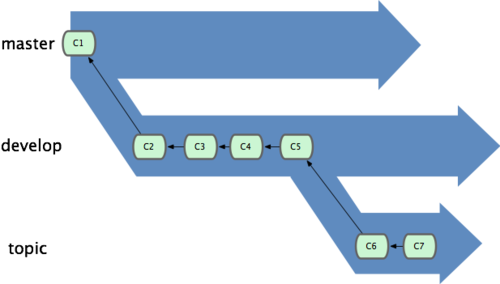
\includegraphics[scale=0.8]{images/branches.png}
\caption{master, develop et topic, trois branches d'un même dépôt.}
\label{branches}
\end{center}
\end{figure}

\emph{La fusion} est l'opération de rassemblement des deux branches en une,
c'est-à-dire dans le cas précédent de regrouper les corrections d'erreurs avec
les nouvelles fonctionnalités.

Les fondamentaux ayant été acquis, j'ai trouvé plusieurs solutions à la
problématique principale qui est la suivante : \newline

Peut-on fusionner des branches tout en choisissant de ne pas fusionner
tout les commits ? \newline

\begin{itemize}
    \item Tout dabord la commande \texttt{git chery-pick nomducommit} permet
    de \og cueillir \fg{} le commit que l'on veut fusionner.
    \item Ensuite on peut aussi rassembler les deux branches puis exécuter la
    commande \texttt{git revert nomducommit} pour inverser les modifications
    du commit après la fusion.
    \item Enfin faire trois branches distinctes pour ne pas avoir à faire les
    opérations ci-dessus\, \footnote{Cette solution à été choisie.}.
\end{itemize}

Git répondant au besoin de l'entreprise, il a fallu que j'effectue des
recherches pour que la migration Subversion\, \footnote{Le logiciel de gestion
de versions le plus utilisé à l'heure actuelle. Il est de type centralisé.}
vers Git se fasse sans perte.

\subsection{L'installation} % (fold)

À peu près au milieu du stage, nous nous sommes heurtés à un problème
technique. Le serveur de l'entreprise ne contenait pas de version récente de
Git. En sachant que celui-ci est mutualisé\, \footnote{L'hébergement mutualisé
est un concept d'hébergement internet destiné principalement à des sites web,
dans un environnement technique dont la caractéristique principale est d'être
partagé par plusieurs utilisateurs. L'administration du ou des serveurs est
assurée par un intervenant tiers tel qu'OVH.}, nous n'avions pas les
autorisations nécessaires pour installer une nouvelle version.

Les logiciels libres sont réputés pour être rétro-compatibles, mais en toute
logique il ne dispose pas des nouveautés sans les mettre à jour. Le problème
est qu'on ne pouvait pas modifier des branches distantes dites \og de suivi
\fg{}. Cette fonctionnalité permet à plusieurs développeurs de travailler en
même temps sur une branche différente de celle par défaut, par exemple pour
expérimenter de nouvelles implémentations à plusieurs. À ce moment-là j'ai été
très déçu et pensais mon travail inutilisable. Cependant, mes efforts n'ont pas
été vain puisque M.\bsc{Dubourg} après quelques recherches, a trouvé sur
internet un utilisateur ayant réussi à installer Git sur un serveur mutualisé.
Nous n'avions pas les droits d'accès aux dossiers des programmes mais rien ne
nous empêchait de compiler Git à partir des sources pour nous permettre de
créer en local le logiciel\, \footnote{Le problème ne se serait pas posé si
j'avais lu le chapitre traitant de la compilation dans mon livre Linux, je n'ai
découvert cette méthode qu'après le stage\dots}. Ceci étant fait, en
redéfinissant la variable système qui stocke les chemins des applications, nous
avons pu utiliser notre compilé dernier cri.

% section L'installation (end)

\subsection{Le passage fatidique} % (fold)

Trois jours avant mon départ, le grand déménagement s'impose. Toute la partie
étude et confection du tutoriel Git prend forme car j'ai basculé tous les
projets qui étaient au préalable sur Subversion vers Git tout en gardant
l'historique des changements provenant de SVN. Après quelques recherches, une
commande Git m'a permis de répondre à ce besoin.\\

\begin{lstlisting}[basicstyle=\ttfamily\small, frame=trBL]
git-svn clone http://svn/repo/here/trunk
\end{lstlisting}
% section Le passage fatidique (end)

\section{Le tutoriel utilisateur} % (fold)
\label{sec:Le tutoriel utilisateur}

Pour aider les développeurs a intégré le nouveau gestionnaire de
version, j'ai élaboré un document Word \copyright{} de quatorze pages
qui explique les bases du logiciel, la mise en place de l'outil dans
leurs environements de travail réspectifs et l'utilisation de celui-ci
avec le gratuiciel TortoiseGit.  Pour être au plus près des
problèmatiques qui pourraient être rencontrés, j'ai conçu l'intégralité
du guide sous forme de questions et de réponses. Sans rentrer dans les
détails, je liste ici les chapitres qui le compose :

\begin{enumerate}
    \item Les bases.
    \item Comment mettre en place Git sur Windows ?
    \item Comment gérer les dépôts Git ?
    \item Comment utiliser Git ?
    \item Comment utiliser les branches ?
    \item Comment consulter l'historique des modifications ?
    \item Quelle est la méthode de travail ?
    \item Annexe.
\end{enumerate}

% section Le tutoriel utilisateur (end)

\section{Les utilitaires} % (fold)

Nous avons longuement discuté sur le côté technique de Git. En effet cet outil
est à la base un logiciel libre provenant de Linux et n'a pas d'interface
graphique, ce choix est établi sur le fait qu'un développeur n'a pas forcément
besoin de cela pour travailler\, \footnote{Sans nul doute que pour un
graphiste, une souris est un élément indispensable pour ses créations, mais pas
pour produire du code.} et aussi que ce logiciel regorge de fonctionnalités et
donc très difficile à simplifier à travers une interface ne pouvant fonctionner
qu'avec une souris. L'équipe n'étant pas très férue de ligne de commande et le
logiciel TortoiseGit reprenant que les fonctions essentielles de Git, il a
fallu que je conçois des petits programmes qui fonctionnent en un clic pour
simplifier les choses répétitives.

% section Introduction (end)

\subsection{Lister les dépôts du serveur}

Mon travail suivant consistait à lister les dépôts Git dans une page PHP\,
\footnote{\emph{Hypertext Preprocessor} est un langage de scripts libre
principalement utilisé pour produire des pages Web dynamiques.}. Le serveur OVH
centralise les codes sources de la société, les développeurs, eux doivent
récupérer une copie des dossiers pour pouvoir travailler dessus. Seulement,
lancer FilleZilla\, \footnote{FileZilla est un logiciel gratuit qui permet de
se connecter à distance sur un serveur pour y télécharger des fichiers.} pour
connaître les noms des répertoires Git puis recopier le bon lien hypertexte
avec le bon chemin d'arborescence est une tâche fastidieuse.  J'ai donc, à
l'aide de mes connaissances en système UNIX, créé un script qui analyse un
dossier défini et qui liste les différents dépôts tout en leurs mettant les
bonnes adresses de téléchargement en préfixe comme nous le montre la figure
\ref{repo}. Du coup, un simple copier-coller du lien du dépôt voulu dans
tortoiseGit suffit pour cloner. Gain de productivité et de simplicité réunie.

\begin{figure}
\begin{center}
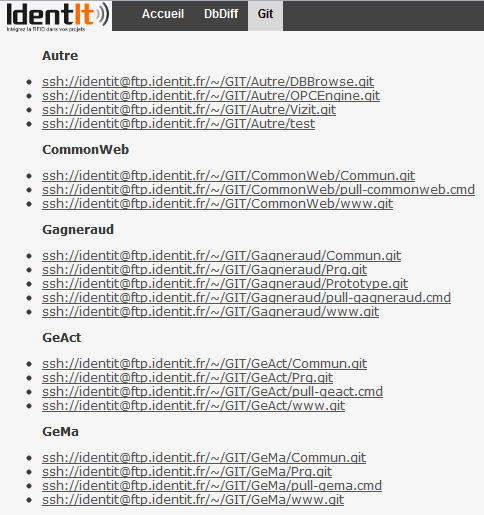
\includegraphics[scale=0.5]{images/repo.png}
\caption{La liste des dépôts cliquables.}
\label{repo}
\end{center}
\end{figure}

% section Mise à jour distante automatique (end)

\subsection{Mise en production automatique} % (fold)

Une fois que les développeurs sont satisfaits de leurs modifications, ils
doivent mettre à jour le dépôt distant pour partager leurs travaux. Une fois
les modifications validées par le chef de projet, celui-ci doit mettre en ligne
sur le dépôt de production. J'ai créé un script Batch \og modèle \fg{} pour
que cela se fasse en un clic.\\

\begin{lstlisting}[basicstyle=\ttfamily\small, frame=trBL]
set PATH=%HOMEPATH%;%PATH%
plink identit@ftp.identit.fr -l identit -pw MOTDEPASSE
"cd LEDOSSIER; git pull; exit;"
\end{lstlisting}

% section Mise en production automatique (end)

\subsection{Mise à jour locale automatique} % (fold)

Les développeurs possèdent des clones des dépôts distants\, \footnote{Ils se
trouvent tous sur le serveur OVH qui sert de point de rencontre comme nous
l'avons vu.} en local pour bien évidemment maintenir le code source. Le fait
qu'il y ait une multitude de dépôts implique une mise à jour des clones locaux
pour récupérer les modifications des autres développeurs ce qui est très
répétitif. J'ai donc créé un script Batch\, \footnote{Désigne un fichier qui
contient une suite de commandes qui seront traitées automatiquement par
Windows\, \copyright.} qui parcourt tous les dossiers englobant les sources des
dépôts et les mets à jour. Pour cela j'ai parcouru la documentation de la
console windows\, et ça n'a pas été évident du tout. Pour l'anecdote, je devais
à partir de mon MacBook\, \footnote{Système de type UNIX.}, lancer une machine
virtuelle Windows\, \footnote{À partir du logiciel VirtualBox.} pour créer mon
script Batch qui s'exécute en console, et qui lance enfin un terminal Linux
pour faire la mise à jour\dots\\

\begin{lstlisting}[basicstyle=\ttfamily\small, frame=trBL]
"C:\Program Files\TortoiseGit\bin\pageant.exe"
C:%HOMEPATH%\.ssh\id_rsa.ppk
"C:\Program Files (x86)\git\bin\sh.exe" --login -i -c
"for i in $(find . -maxdepth 2 -mindepth 2 -type d);
do
    cd $i;
    echo $i;
    git remote -v;
    git pull; cd ../..;
done"
\end{lstlisting}

\clearpage
